% ------------------------------------------------------------------
% NAACL 2027 System Demonstrations -- DocResolve: outline / skeleton
% Paste into Overleaf next to acl.sty + acl_natbib.bst (ACL template).
% Page budget (6 pages + references; Limitations/Ethics do not count):
%   Abstract 0.25 | Introduction 0.75 | Related Work 0.5
%   System Architecture 1.5 | System Demonstration 1.5
%   Empirical Evaluation 1.25 | Conclusion 0.25
% Every \todo{} is a note to ourselves; remove before submission.
% [auto] = automatic metric from the Mac runs; [judge] = from the H200 run.
%
% FIGURE AND TABLE PLAN (where, what, how it is made)
%   Fig 1  Introduction, one column   result view screenshot, annotated 1-5
%   Fig 2  Architecture, full width   method diagram (TikZ below, no image)
%   Fig 3  Demonstration, full width  reader: answer doc + dissent doc side by
%                                     side with highlights; corroboration strip
%   Fig 4  Demonstration, one column  governance override before/after (2 panels)
%   Fig 5  Evaluation, one column     accuracy vs misinformation scatter, RAMDocs
%                                     (figures/fig_tradeoff_ramdocs.pdf)
%   Fig 6  Evaluation, full width     decision mix per system, both benchmarks
%                                     (figures/fig_decisions.pdf)
%   Fig 7  Evaluation, one column     RAMDocs set-EM on items with / without
%                                     planted misinformation (figures/fig_slices_ramdocs.pdf)
%   Fig 8  Evaluation or appendix     CONFLICTS accuracy by conflict type, heatmap
%                                     (figures/fig_conflict_types.pdf)
%   Tab 1  Evaluation, full width     accuracy, systems x three generators
%   Tab 2  Evaluation, full width     behaviour under the main generator
%   Tab 3  Evaluation (after judging) FC / PC / Inc per system and generator
%   Charts are produced by paper/figures/make_charts.py from results_external/.
% ------------------------------------------------------------------
\documentclass[11pt]{article}
\usepackage[final]{acl}           % demo track is not anonymous: authors shown
                                  % (use [review] only if the call asks for line numbers)
\usepackage{times}
\usepackage{latexsym}
\usepackage{booktabs}
\usepackage{graphicx}
\usepackage{xcolor}
\usepackage{microtype}
\usepackage{inconsolata}
\usepackage{tikz}
\usetikzlibrary{arrows.meta,positioning,fit,backgrounds,calc}
\usepackage{listings}
\graphicspath{{figures/}}

% ---- verbatim prompt boxes (appendix) ----------------------------------
\lstdefinestyle{prompt}{
  basicstyle=\ttfamily\scriptsize, columns=fullflexible, keepspaces=true,
  breaklines=true, breakindent=0pt, breakautoindent=false,
  frame=single, framerule=0.3pt, rulecolor=\color{boxline},
  backgroundcolor=\color{boxfill}, xleftmargin=4pt, xrightmargin=4pt,
  aboveskip=4pt, belowskip=8pt, showstringspaces=false,
  literate={->}{{$\rightarrow$}}2}

% ---- one-line switch for the system name -------------------------
\newcommand{\sysname}{DocResolve}   % decided 24 Nov 2026
\newcommand{\todo}[1]{\textcolor{red}{[TODO: #1]}}
\newcommand{\tbd}{\textcolor{red}{--}}   % number not yet available
% ---- the three generator models (column groups of Table 1) ---------
\newcommand{\genA}{Nemotron 3.5 Super}
\newcommand{\genB}{\todo{model B}}
\newcommand{\genC}{\todo{model C}}

% ---- colours shared by the diagram and the UI ------------------------
\definecolor{support}{HTML}{1F7A4D}   % committed answer / supporting evidence
\definecolor{dissent}{HTML}{B7791F}   % flagged dissent
\definecolor{context}{HTML}{6B7280}   % retrieved, not cited
\definecolor{boxfill}{HTML}{F4F7F5}
\definecolor{boxline}{HTML}{9BB4A4}

\title{\sysname: Conflict-Aware Question Answering\\that Answers and Flags the Dissent}

\author{Gaurav Najpande \\
        Arizona State University \\
        \texttt{\todo{asurite}@asu.edu} \And
        Vivek Gupta \\
        Arizona State University \\
        \texttt{\todo{asurite}@asu.edu}}

\begin{document}
\maketitle

% ==================================================================
\begin{abstract}
\todo{0.25 page, about 150 words, four sentences.}
(1) Problem: in real document collections the retrieved passages disagree
(superseded policies, drafts, summaries that lag the source, neighbouring
scopes); RAG systems either pick a value silently, usually the majority one,
or refuse to answer.
(2) System: \sysname{} commits to an answer, flags the dissent, shows how
many independent documents back each competing value, and traces every
claim to a highlighted sentence in the original file; a reviewer can
override a document's status and watch the answer re-evaluate.
(3) Evidence: on RAMDocs and CONFLICTS with the same generator, the
answer-and-flag policy recovers the accuracy lost by refusing on conflict
(RAMDocs set-EM 45.6 vs 38.2 for refuse-on-conflict and 41.4 for plain RAG
[auto]; misinformation-in-answer 23.8 vs 35.0 [auto]) \todo{replace with
judge FC/Inc once available}.
(4) Availability: open-source, \texttt{pip install docresolve}, runs
against any OpenAI-compatible endpoint; demo at \todo{URL}; video at
\todo{URL}.
\end{abstract}

% ==================================================================
\section{Introduction}
\todo{0.75 page. Figure 1 sits here.}
\begin{itemize}
  \item Opening scene: one question, five documents, four different numbers
        (the Meridian Forge defect-rate example from the demo: 0.72\% in the
        active bulletin vs 1.00\% in five summaries, drafts and an
        out-of-scope audit note). This is the normal state of an enterprise
        knowledge base, not an edge case.
  \item Two failure modes of conventional RAG under conflicting evidence:
        (a) \emph{silent majority}: the generator follows the most repeated
        value, which is how stale and wrong values win; (b) \emph{refusal}:
        conflict-aware systems that abstain whenever sources disagree are
        safe but useless for the questions people actually ask. Our own
        refuse-on-conflict variant loses 7 points of set-EM on RAMDocs to
        this [auto].
  \item What a practitioner needs instead: a committed answer, the dissent
        made visible, a reason the system chose one value over another, and
        the exact sentence each claim came from so the decision can be
        checked in seconds.
  \item Contributions, four bullets:
        (1) an \emph{answer-and-flag} resolution policy with a fixed rule
        order (governance $\rightarrow$ corroboration by distinct documents
        $\rightarrow$ internal consistency $\rightarrow$ declared tie) and
        verbatim-quote validation;
        (2) an evidence-review interface that renders the committed answer,
        the flagged dissent, per-value corroboration counts and
        sentence-level highlights in the original PDF/Word/text file, with
        reviewer overrides of document status;
        (3) a pip-installable package and server that run the same pipeline
        over a folder, an upload, or a server-side path, against any
        OpenAI-compatible model;
        (4) an evaluation on two public conflict benchmarks and three
        generators against plain, hybrid and refuse-on-conflict RAG and
        off-the-shelf frameworks, with an LLM-judge protocol.
\end{itemize}

\begin{figure}[t]
  \centering
  \fbox{\parbox{0.95\columnwidth}{\centering\vspace{2.2cm}\todo{Fig 1: result
  view screenshot. Crop to the answer card: (1) decision badge, (2) answer,
  (3) resolution rule, (4) corroboration strip 0.72\% $\times$1 green vs
  1.00\% $\times$5 amber, (5) citations coloured by role.}\vspace{2.2cm}}}
  \caption{\sysname{} on a question whose sources disagree: a committed
  answer, the rule that decided it, how many documents back each competing
  value, and the dissent flagged rather than hidden.}
  \label{fig:teaser}
\end{figure}

% ==================================================================
\section{Related Work}
\todo{0.5 page, three paragraphs; cite, do not survey.}
\begin{itemize}
  \item \textbf{Conflict-aware RAG.} Taxonomies and benchmarks: CONFLICTS
        (Cattan et al.\ 2025), ConflictBank, RAMDocs / MADAM-RAG (Wang et
        al.\ 2025), ConfRAG (ACL 2026). Methods: multi-agent debate
        (MADAM-RAG), conflict-driven summarisation (CARE-RAG),
        detect-classify-resolve pipelines (ConflictRAG), transparent conflict
        handling (TCR, AAAI 2026). Position: these optimise the answer; none
        ship an interface where a person can see \emph{why} one value won
        and overrule it. \todo{re-check for 2026 demos on the same topic.}
  \item \textbf{Evidence attribution.} Verbatim quoting and post-hoc
        citation checking (\todo{ALCE, quote-verification work}). We require
        verbatim quotes, validate them against the retrieved chunk, repair
        once, and map them to character spans in the source document.
  \item \textbf{Governance-aware retrieval.} Authority, recency and
        provenance signals in enterprise search and document QA
        (\todo{cites}); off-the-shelf stacks (LlamaIndex, Rankify, Open
        WebUI), also our baselines, treat the corpus as consistent.
\end{itemize}

% ==================================================================
\section{System Architecture}
\todo{1.5 pages. Figure 2 (method diagram) at the top of the section.}

\begin{figure*}[t]
\centering
\resizebox{\textwidth}{!}{%
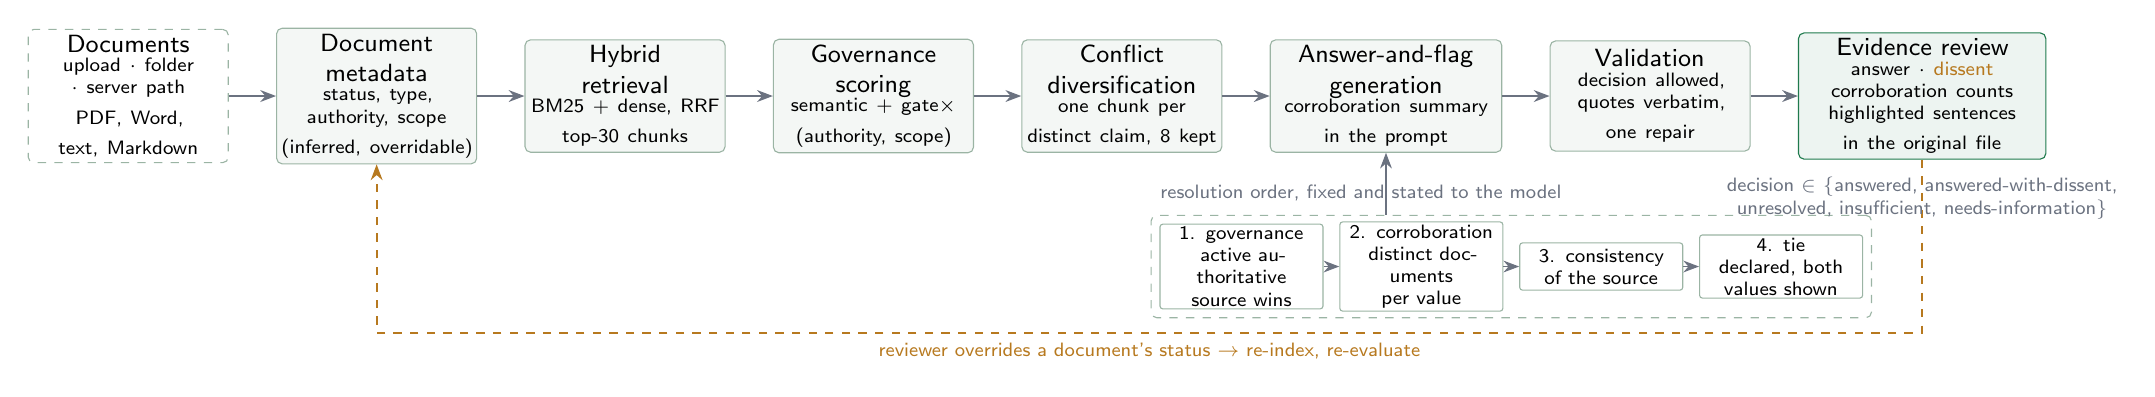
\begin{tikzpicture}[
  font=\sffamily\small,
  node distance=5mm and 6mm,
  stage/.style={draw=boxline, fill=boxfill, rounded corners=2pt, align=center,
                minimum height=14mm, text width=24mm, inner sep=2pt},
  io/.style={stage, fill=white, dashed},
  ui/.style={stage, draw=support, fill=support!8, text width=30mm},
  rule/.style={draw=boxline, fill=white, rounded corners=1pt, align=center,
               text width=20mm, minimum height=6mm, inner sep=1pt, font=\sffamily\scriptsize},
  arr/.style={-{Stealth[length=2mm]}, thick, draw=context},
  lbl/.style={font=\sffamily\scriptsize, text=context, align=center},
]
% ---- main pipeline, left to right ------------------------------------
\node[io] (docs) {Documents\\[-1pt]{\scriptsize upload $\cdot$ folder $\cdot$ server path\\PDF, Word, text, Markdown}};
\node[stage, right=of docs] (meta) {Document\\metadata\\[-1pt]{\scriptsize status, type, authority, scope\\(inferred, overridable)}};
\node[stage, right=of meta] (retr) {Hybrid\\retrieval\\[-1pt]{\scriptsize BM25 + dense, RRF\\top-30 chunks}};
\node[stage, right=of retr] (score) {Governance\\scoring\\[-1pt]{\scriptsize semantic + gate$\times$\\(authority, scope)}};
\node[stage, right=of score] (div) {Conflict\\diversification\\[-1pt]{\scriptsize one chunk per\\distinct claim, 8 kept}};
\node[stage, right=of div, text width=28mm] (gen) {Answer-and-flag\\generation\\[-1pt]{\scriptsize corroboration summary\\in the prompt}};
\node[stage, right=of gen] (val) {Validation\\[-1pt]{\scriptsize decision allowed,\\quotes verbatim,\\one repair}};
\node[ui, right=of val] (ui) {Evidence review\\[-1pt]{\scriptsize answer $\cdot$ \textcolor{dissent}{dissent}\\corroboration counts\\highlighted sentences\\in the original file}};
\foreach \a/\b in {docs/meta, meta/retr, retr/score, score/div, div/gen, gen/val, val/ui}
  \draw[arr] (\a) -- (\b);
% ---- resolution order under the generator -----------------------------
\node[rule, below=9mm of gen.south west, anchor=north west, xshift=-14mm] (r1) {1. governance\\active authoritative\\source wins};
\node[rule, right=2mm of r1] (r2) {2. corroboration\\distinct documents\\per value};
\node[rule, right=2mm of r2] (r3) {3. consistency\\of the source};
\node[rule, right=2mm of r3] (r4) {4. tie\\declared, both\\values shown};
\foreach \a/\b in {r1/r2, r2/r3, r3/r4} \draw[arr, thin] (\a) -- (\b);
\begin{scope}[on background layer]
  \node[draw=boxline, dashed, rounded corners=2pt, fit=(r1)(r4), inner sep=3pt] (rules) {};
\end{scope}
\node[lbl, above=0.5mm of rules.north west, anchor=south west] {resolution order, fixed and stated to the model};
\draw[arr, thin] (rules.north -| gen.south) -- (gen.south);
% ---- reviewer override loop ---------------------------------------------
\draw[arr, draw=dissent, dashed] (ui.south) -- ++(0,-22mm) -| (meta.south)
  node[lbl, pos=0.25, below, text=dissent] {reviewer overrides a document's status $\rightarrow$ re-index, re-evaluate};
% ---- output legend on the right ------------------------------------------
\node[lbl, below=1mm of ui] {decision $\in$ \{answered, answered-with-dissent,\\unresolved, insufficient, needs-information\}};
\end{tikzpicture}}
\caption{\sysname{} pipeline. Documents enter with inferred governance
metadata; hybrid retrieval and governance-weighted scoring select chunks;
conflict diversification guarantees the generator sees every competing
value; generation follows a fixed resolution order and must quote verbatim;
validation repairs or downgrades invalid outputs; the interface shows the
committed answer with its dissent and lets a reviewer override document
status, which re-runs the pipeline.}
\label{fig:pipeline}
\end{figure*}

\subsection{Retrieval}
\begin{itemize}
  \item Inputs: file upload, whole-folder upload with paths kept, or a
        server-side folder path (mounted share, export); PDF, Word, text,
        Markdown. Folder structure becomes the document path shown in
        citations. Chunking is paragraph/sentence based; chunk and page
        offsets are kept for highlighting.
  \item Hybrid retrieval: BM25 and dense (bge-small) fused by reciprocal rank,
        top-30. Why hybrid: policy and version identifiers (``Tier-B'',
        ``Q4-certified'', dates) are lexical; the ablation shows the gain is
        real only on top of the answer-and-flag policy [auto: 45.6 vs 43.6].
\end{itemize}

\subsection{Authority and scope scoring}
\begin{itemize}
  \item Per-document metadata inferred from text: \emph{status}
        (active-authoritative, active, draft, superseded, archived, unknown),
        \emph{document type}, an \emph{authority} score, scope cues.
        Reviewer overrides are stored next to the inferred values and shown
        to the model as ``set by reviewer''.
  \item Score $= 0.3\cdot\text{semantic} + g\cdot(0.5\cdot\text{authority} +
        0.2\cdot\text{scope})$; the gate $g$ applies governance weight only
        when the chunk carries governance signals, so on corpora without them
        (the public benchmarks) the scorer degrades to semantic ranking.
        \todo{state exactly as implemented in \texttt{core.py}.}
\end{itemize}

\subsection{Conflict resolution}
\begin{itemize}
  \item Conflict diversification: group chunks by the numeric/categorical
        claim they make, keep one chunk per distinct claim first, then fill
        to 8, so the generator always sees the competing values rather than
        eight copies of the majority one.
  \item Prompt receives chunks with status, type, authority and a
        \emph{corroboration summary} (how many distinct documents state each
        value). Resolution order, fixed and stated: (1) governance;
        (2) corroboration by distinct documents, not repeated chunks of one
        document; (3) internal consistency; (4) a declared tie.
  \item Output schema: decision $\in$ \{answered, answered-with-dissent,
        unresolved-conflict, insufficient-evidence, needs-information\},
        short answer(s), explanation, resolution rule, citations with
        verbatim quotes and roles (support / dissent / context).
\end{itemize}

\subsection{Dissent attribution}
\begin{itemize}
  \item Validation: allowed decision, every quote verbatim in its chunk under
        normalised matching; one repair round; salvage to the most
        conservative valid decision if repair fails. Invalid outputs after
        repair: 0 and 1 for \sysname{} vs 5 and 88 for plain RAG [auto].
  \item Span location: each verified quote is mapped to character offsets in
        the chunk and in the full document (ellipsis segments allowed), and
        to a page for PDFs; the interface only marks ranges, it never
        re-searches text. Citations carry a role so support and dissent are
        coloured differently everywhere.
\end{itemize}

% ==================================================================
\section{System Demonstration}
\todo{1.5 pages. Figures 3 and 4. Write as a walkthrough the video follows.}

\subsection{Interface}
\begin{itemize}
  \item \textbf{Evidence review.} Decision badge (``Answered $\cdot$ dissent
        flagged''), the answer, model-reported confidence, the resolution
        panel (rule + one-sentence summary), the corroboration strip (each
        competing value, number of distinct documents, green for the
        committed value, amber for the rest), citations coloured by role.
  \item \textbf{Where the answer comes from.} Clicking a citation opens the
        document beside the results with the cited sentence highlighted and
        chunk boundaries drawn; ``Compare side by side'' opens the dissenting
        document underneath. Text view by default; an Original tab renders
        the actual PDF page (pdf.js text layer) or the Word file with the
        same highlight.
  \item \textbf{Governance in the loop.} The document tree shows inferred
        status and type per file with dropdowns to override; an override
        re-indexes, nudges the authority score, and is shown to the model as
        a reviewer decision.
  \item \textbf{Record.} Footer with model, retrieval, policy, latency; a
        ``Download record'' export (question, decision, resolution, citations
        with spans, document metadata) for audit.
\end{itemize}

\begin{figure*}[t]
  \centering
  \fbox{\parbox{0.97\textwidth}{\centering\vspace{3cm}\todo{Fig 3: full
  workspace screenshot. Left: result card with corroboration strip. Right:
  reader with the policy bulletin (0.72\% sentence in green) above the
  operations handbook (1.00\% sentence in amber), chunk boundary visible.
  Annotate the Original tab.}\vspace{3cm}}}
  \caption{The evidence review. The committed value and the dissenting value
  are each traced to the sentence they come from, shown side by side in the
  source documents.}
  \label{fig:reader}
\end{figure*}

\subsection{User workflow}
\begin{enumerate}
  \item Create a collection; upload files, drop a folder, or type a server
        folder path (a mounted share or knowledge-base export). The tree
        shows every file with its inferred status and type.
  \item Ask a question, optionally with case context (date, region, employee
        category). Get the committed answer with the dissent flagged.
  \item Open the cited sentences in the original files; compare the
        dissenting document side by side.
  \item Disagree with a document's status? Override it; the answer is
        re-evaluated and the override is recorded.
  \item Download the record.
\end{enumerate}

\subsection{Illustrative examples}
\begin{itemize}
  \item \textbf{Governance decides.} Meridian Forge defect rate: five
        documents say 1.00\%, one active bulletin says 0.72\%; the system
        answers 0.72\% by governance and shows 1.00\% $\times$5 as dissent.
  \item \textbf{Corroboration decides.} Mark the bulletin superseded: the
        answer moves to 1.00\% by corroboration (5 documents), dissent still
        flagged, override shown in technical details (Figure~\ref{fig:override}).
  \item \textbf{Mixed formats.} Remote-work policy (PDF, page 2) vs a 2024 FAQ
        (Word): 3 days vs 2 days, resolved by governance, each sentence
        highlighted on the real page.
  \item \textbf{Walkthrough corpus.} The 180-document fictional policy pack
        (15 questions $\times$ 12 documents, each with an authoritative source
        and typed distractors: superseded, draft, secondary summary,
        neighbouring scope, background note). Demo only; not in the tables.
\end{itemize}

\begin{figure}[t]
  \centering
  \fbox{\parbox{0.95\columnwidth}{\centering\vspace{1.8cm}\todo{Fig 4: two
  stacked panels. Top: bulletin active, answer 0.72\%, rule governance.
  Bottom: bulletin set to superseded by reviewer, answer 1.00\%, rule
  corroboration, 5 documents.}\vspace{1.8cm}}}
  \caption{A reviewer override changes which rule decides. The dissent stays
  visible in both cases.}
  \label{fig:override}
\end{figure}

% ==================================================================
\section{Empirical Evaluation}
\todo{1.25 pages. Tables 1 and 2, Figures 5 to 7; Figure 8 to the appendix
if space is short.}

\subsection{Existing datasets}
\begin{itemize}
  \item RAMDocs (500 questions; ambiguity, noise and misinformation mixed per
        question; metric: set exact match over the gold answer set, plus
        \emph{misinformation-in-answer}). CONFLICTS (458 questions;
        expert-annotated conflict types with an expected behaviour per type;
        metric: answer containment and decision match). Neither carries
        governance metadata, so the governance rule is inert here and the
        comparison isolates retrieval + policy. \todo{say this plainly; it
        pre-empts the obvious reviewer question.}
\end{itemize}

\subsection{Baselines and metrics}
\begin{itemize}
  \item \textbf{Generators.} \genA, \genB, \genC; local bge-small embeddings;
        identical prompts and decoding within a column group. \todo{temperature,
        max tokens, endpoints.}
  \item \textbf{Systems.} \sysname{} (hybrid, answer-and-flag); ablations:
        dense + answer-and-flag, hybrid + refuse-on-conflict, dense +
        refuse-on-conflict (the original strict system); controls: hybrid RAG
        and dense RAG with the same retriever and no policy, closed-book;
        off-the-shelf: LlamaIndex ($k{=}2,8$), Rankify, Open WebUI.
  \item \textbf{LLM judge.} Three-way grading (fully correct / partially
        correct / incorrect, SentryLine convention) by one open-weight judge
        outside the generators' families (\todo{Qwen3-32B or gpt-oss-120b},
        self-hosted with vLLM); every row judged once. Sanity check: agreement
        with an earlier GLM judge on six rows, and with gold on a labelled
        subset. \todo{numbers from compare\_with\_glm.py.}
\end{itemize}

\subsection{Results}
Table~\ref{tab:main} is the headline: every system under each generator,
one accuracy number per benchmark. Table~\ref{tab:behaviour} explains the
headline for the main generator: how often each system commits to a wrong
value, how often it refuses, and what it costs.
Figure~\ref{fig:tradeoff} shows the same trade-off in one picture;
Figure~\ref{fig:decisions} the decision mix; Figure~\ref{fig:slices} where the
gain comes from. \todo{once the judge has run, add Table 3 with FC / PC / Inc
per generator and move the headline to FC.}

% ---------------- Table 1: accuracy across three generators ----------
\begin{table*}[t]
\centering
\small
\setlength{\tabcolsep}{5pt}
\begin{tabular}{@{}l cc cc cc@{}}
\toprule
 & \multicolumn{2}{c}{\genA} & \multicolumn{2}{c}{\genB} & \multicolumn{2}{c}{\genC} \\
\cmidrule(lr){2-3} \cmidrule(lr){4-5} \cmidrule(lr){6-7}
 & RAMDocs & CONFLICTS & RAMDocs & CONFLICTS & RAMDocs & CONFLICTS \\
 & set-EM & contain. & set-EM & contain. & set-EM & contain. \\
\midrule
\textbf{\sysname{}} (hybrid retrieval, answer-and-flag)
                                  & \textbf{45.6} & 74.7 & \tbd & \tbd & \tbd & \tbd \\
\addlinespace[2pt]
\multicolumn{7}{@{}l}{\emph{Ablations}} \\
\quad dense retrieval, answer-and-flag     & 43.6 & 74.3 & \tbd & \tbd & \tbd & \tbd \\
\quad hybrid retrieval, refuse-on-conflict & 37.6 & 76.0 & \tbd & \tbd & \tbd & \tbd \\
\quad dense retrieval, refuse-on-conflict  & 38.2 & 71.7 & \tbd & \tbd & \tbd & \tbd \\
\addlinespace[2pt]
\multicolumn{7}{@{}l}{\emph{Controls (same retriever and generator, no policy)}} \\
\quad hybrid RAG                           & 41.6 & 77.2 & \tbd & \tbd & \tbd & \tbd \\
\quad dense RAG                            & 41.4 & 65.4 & \tbd & \tbd & \tbd & \tbd \\
\quad closed-book                          &  8.6 & 58.2 & \tbd & \tbd & \tbd & \tbd \\
\addlinespace[2pt]
\multicolumn{7}{@{}l}{\emph{Off-the-shelf frameworks}} \\
\quad LlamaIndex, $k{=}2$                  & 23.8 & 62.9 & \tbd & \tbd & \tbd & \tbd \\
\quad LlamaIndex, $k{=}8$                  & 39.6 & 74.7 & \tbd & \tbd & \tbd & \tbd \\
\quad Rankify                              & 42.8 & \textbf{78.1} & \tbd & \tbd & \tbd & \tbd \\
\quad Open WebUI$^\dagger$                 & 40.3 & --   & \tbd & \tbd & \tbd & \tbd \\
\bottomrule
\end{tabular}
\caption{Accuracy under three generators. RAMDocs (500 questions): set exact
match over the gold answer set. CONFLICTS (458 questions): answer containment.
Retrieval, prompts and decoding are identical within a column group; only the
generator changes across groups. Best per column in bold.
$^\dagger$462 of 500 RAMDocs items. \todo{fill \genB{} and \genC{}. Decide
whether Rankify's containment counts as a fair comparison (it returns free
text, no decision).}}
\label{tab:main}
\end{table*}

% ---------------- Table 2: behaviour under the main generator -----------
\begin{table*}[t]
\centering
\small
\setlength{\tabcolsep}{5pt}
\begin{tabular}{@{}l c cc cc cc@{}}
\toprule
 & misinfo in & \multicolumn{2}{c}{refused} & \multicolumn{2}{c}{invalid outputs} & \multicolumn{2}{c}{latency (s)} \\
 & answer$\downarrow$ & \multicolumn{2}{c}{(of 500 / 458)} & \multicolumn{2}{c}{after repair} & \multicolumn{2}{c}{per question} \\
\cmidrule(lr){2-2} \cmidrule(lr){3-4} \cmidrule(lr){5-6} \cmidrule(lr){7-8}
 & RAMDocs & RAMDocs & CONFL. & RAMDocs & CONFL. & RAMDocs & CONFL. \\
\midrule
\textbf{\sysname{}}                        & 23.8 &  45 &  30 & 0 &  1 & 37 & 57 \\
\addlinespace[2pt]
\quad dense retrieval, answer-and-flag     & \textbf{23.0} &  45 &  35 & 1 &  0 & 51 & 75 \\
\quad hybrid retrieval, refuse-on-conflict & 36.6 &  96 & 122 & 0 &  2 & 54 & 65 \\
\quad dense retrieval, refuse-on-conflict  & 35.0 &  99 & 155 & 0 & 39 & 33 & 40 \\
\addlinespace[2pt]
\quad hybrid RAG                           & 26.2 &  44 &  29 & 1 &  0 & 25 & 51 \\
\quad dense RAG                            & 26.0 &  39 & 114 & 5 & 88 & 31 & 41 \\
\quad closed-book                          &  3.6 & 191 &  46 & 0 &  0 & 21 & 40 \\
\addlinespace[2pt]
\quad LlamaIndex, $k{=}2$ / $k{=}8$        & 34.4 / 37.8 & -- & -- & -- & -- & 55 / 12 & 4 / 128 \\
\quad Rankify                              & 28.6 & -- & -- & -- & -- & 45 & 22 \\
\quad Open WebUI$^\dagger$                 & 42.6 & -- & -- & -- & -- & 23 & -- \\
\bottomrule
\end{tabular}
\caption{What the headline hides, main generator (\genA). \emph{Misinfo in
answer}: share of RAMDocs answers that present a planted wrong value as the
answer. \emph{Refused}: unresolved-conflict + insufficient-evidence +
needs-information decisions. \emph{Invalid outputs}: responses that still
failed schema or quote validation after one repair. Off-the-shelf frameworks
return free text, so they have no decisions or validation. Closed-book
``refuses'' by saying it does not know. \todo{consider splitting
\emph{refused} into unresolved-conflict (\sysname{}: 36 / 8) and
insufficient-evidence.}}
\label{tab:behaviour}
\end{table*}

\begin{figure}[t]
  \centering
  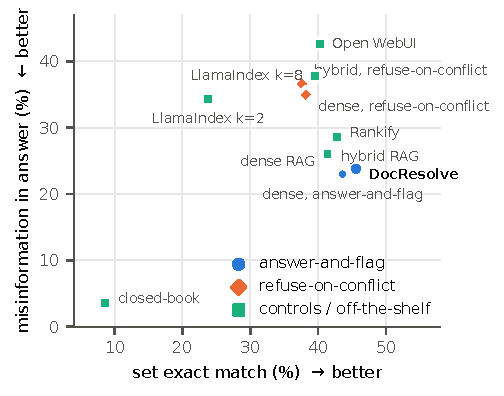
\includegraphics[width=\columnwidth]{fig_tradeoff_ramdocs}
  \caption{RAMDocs: accuracy against misinformation-in-answer, one point per
  system (\genA). The answer-and-flag systems are the only ones that gain
  accuracy without repeating planted misinformation more often.}
  \label{fig:tradeoff}
\end{figure}

\begin{figure*}[t]
  \centering
  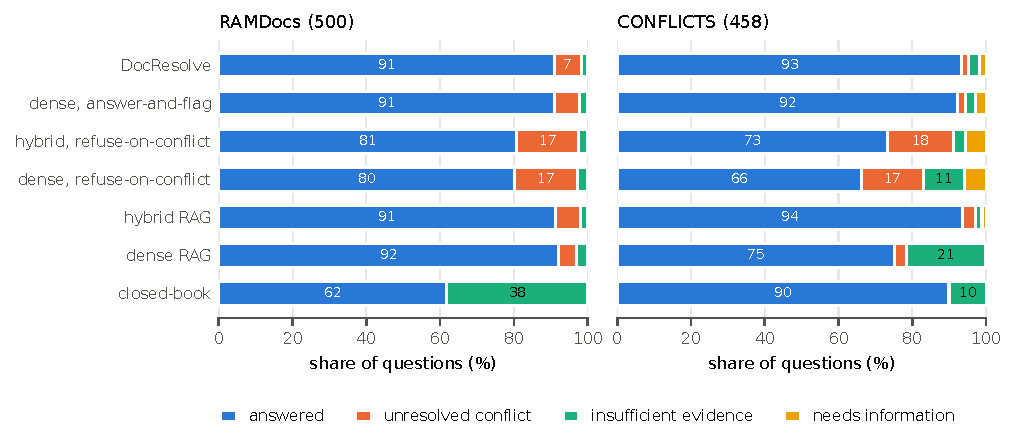
\includegraphics[width=\textwidth]{fig_decisions}
  \caption{Decision mix per system on both benchmarks (\genA). Refuse-on-conflict
  turns a fifth to a third of the questions into refusals; \sysname{} answers
  them and marks the dissent instead.}
  \label{fig:decisions}
\end{figure*}

\begin{figure}[t]
  \centering
  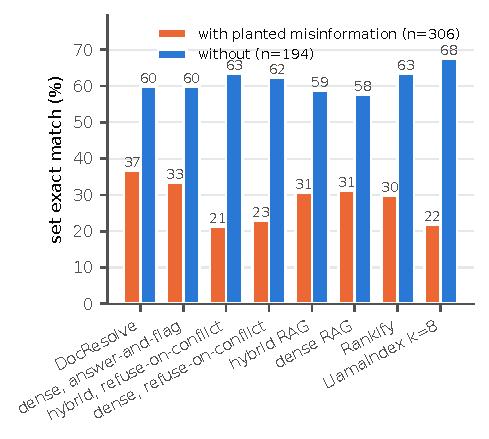
\includegraphics[width=\columnwidth]{fig_slices_ramdocs}
  \caption{RAMDocs set-EM on questions with and without planted misinformation
  (\genA). On clean questions every system is within a few points; the
  difference is entirely on the questions where sources disagree.}
  \label{fig:slices}
\end{figure}

\todo{Analysis paragraphs: (1) the strict system's deficit is the refusal
policy, not retrieval (misinfo slice 22.9 $\rightarrow$ 36.6; paired wins
39/18 vs plain RAG, 54/17 vs strict [auto]); (2) the CONFLICTS 74.7 vs 77.2
gap against hybrid RAG is real and must be discussed: containment counts a
refusal that mentions the gold value as a hit (hybrid refuse-on-conflict
reaches 76.0 while refusing 122 times), which is why the judge's FC / Inc
columns carry the final claim; (3) cost: one extra generation call at most,
57 s vs 51 s on CONFLICTS.}

% ==================================================================
\section{Conclusion}
\todo{0.25 page. Contributions in three sentences, then the three
limitations that matter most, then availability: \texttt{pip install
docresolve}, CLI, server, any OpenAI-compatible endpoint, licence,
repository, demo and video URLs.}

% ==================================================================
\section*{Limitations}
\todo{Required section, outside the page budget. Be concrete.}
\begin{itemize}
  \item Governance signals are inferred from document text; on the public
        benchmarks they are absent, so the governance rule is evaluated only
        through the demo corpus, not the tables.
  \item One judge; results may shift with other judges. The judge is
        open-weight and the protocol is released.
  \item Highlighting in PDFs depends on a text layer; scanned or two-column
        PDFs fall back to the text view.
  \item Latency of roughly a minute per question with the hosted generator;
        acceptable for review workflows, not for chat.
  \item English only; numeric and categorical conflicts are the ones the
        diversification step detects best.
\end{itemize}

\section*{Ethics Statement}
\todo{Short: no personal data in the benchmarks or the demo pack; the
fictional pack contains invented companies; the system surfaces
disagreement rather than hiding it, but a committed answer is still a
model output and the interface is built so a person checks it.}

\section*{Acknowledgements}
\todo{compute (H200), funding, the EMNLP workshop lineage if desired.}

\bibliography{references}
\bibliographystyle{acl_natbib}

% ==================================================================
\appendix
\section{Prompts}
\label{app:prompts}
All prompts are reproduced verbatim from the released code
(\texttt{docuinsight/core.py}). Every system below receives the same user turn
(Appendix~\ref{app:user-turn}) and must return the same JSON schema, so rows
differ only in the system prompt, the retriever and the policy. Decoding is
greedy (temperature 0) with a 16\,384-token completion budget for every
generator.

\subsection{\sysname{}: answer-and-flag system prompt}
\label{app:prompt-flag}
\begin{lstlisting}[style=prompt]
You answer questions using only the supplied evidence passages and optional case context.
Read full passages, including conditions and exceptions. Never infer organizational authority
as verified fact: status, document type, authority scores, and scope similarity are inferred
signals only; scope similarity is not proof of applicability. Never invent precedence.

Choose exactly one decision:
- answered: evidence supports a direct answer, including its conditions and exceptions.
- unresolved_conflict: applicable passages disagree AND the competing values are equally
  supported (see the tie rule below).
- needs_information: relevant rules exist, but essential facts about this case are missing.
- insufficient_evidence: retrieved passages do not support an answer.

Resolving disagreement, in order:
1. Governance: a passage that is explicitly superseded, out of scope, or supporting context
   does not compete. A document saying it "supersedes" earlier documents is not itself superseded.
2. Corroboration: among the passages that do compete, prefer the value supported by more
   independent documents (different filenames). Treat the "Corroboration" summary, when
   supplied, as a count aid only; verify it against the passages.
3. Consistency: prefer the value that agrees with the other facts in the evidence (dates,
   places, names, totals) and that comes from a more specific, internally consistent passage.
4. Tie rule: only if the competing values are supported by the same number of independent
   documents and steps 1 and 3 do not separate them, choose unresolved_conflict.

When you commit under step 2 or 3, the decision is answered, conflict_detected is true, the
dissenting passage is cited with treatment "conflicting", and the explanation names the
rejected value and why it lost. short_answers must contain only the committed answer(s), never
the rejected value. If the question is ambiguous because several distinct entities share the
same name, give the correct answer for each entity; that is not a conflict.

Return JSON only:
{
  "decision": "answered|unresolved_conflict|needs_information|insufficient_evidence",
  "answer": "Readable answer with all important conditions and exceptions; mention flagged dissent briefly.",
  "short_answers": ["each distinct final answer as a short span; for an unresolved conflict, each competing answer"],
  "citations": [
    {"chunk_id": "exact supplied chunk id", "quote": "verbatim excerpt from that passage",
     "treatment": "governing|supporting|superseded|different_scope|conflicting|uncertain",
     "explanation": "brief plain-language treatment"}
  ],
  "explanation": "Brief explanation of this decision, including how any conflict was resolved.",
  "missing_information": [],
  "clarification_question": null,
  "selected_source": null,
  "conflict_detected": false,
  "confidence": "high|medium|low"
}
For unresolved conflicts, cite each materially competing passage and explain its treatment;
selected_source must be null. For needs_information, list the missing facts and ask a useful
clarification question. Use an empty citation list if evidence cannot support any citation.
When the decision is answered, selected_source must be the filename of the governing passage the
answer is taken from (never null). selected_source must exactly match a supplied filename and
appear in citations. Numeric claim metadata is a search aid, never a citation or proof.
\end{lstlisting}

\subsection{Refuse-on-conflict system prompt (ablation)}
\label{app:prompt-strict}
Identical to Appendix~\ref{app:prompt-flag} except for the decision list and
the absence of the resolution order; the JSON schema and the closing
instructions are the same. The differing block:
\begin{lstlisting}[style=prompt]
Choose exactly one decision:
- answered: evidence supports a direct answer, including its conditions and exceptions.
- unresolved_conflict: applicable evidence disagrees and documented precedence does not resolve it.
- needs_information: relevant rules exist, but essential facts about this case are missing.
- insufficient_evidence: retrieved passages do not support an answer.

Do not force a winner between equally applicable conflicting passages. Distinguish different
scope, explicitly superseded material, supporting context, and uncertain applicability. A
document saying it "supersedes" earlier documents is not itself superseded.
\end{lstlisting}

\subsection{Plain RAG system prompt (controls)}
\label{app:prompt-baseline}
Used by the dense-RAG and hybrid-RAG controls: same schema, no governance or
conflict guidance, and the evidence blocks omit the inferred signal lines.
\begin{lstlisting}[style=prompt]
You answer questions using only the supplied evidence passages and optional case context.
Read the passages and answer the question as directly as you can from them. If the passages
disagree, use your best judgment about which answer the evidence supports.

Return JSON only:
{
  "decision": "answered|unresolved_conflict|needs_information|insufficient_evidence",
  "answer": "Readable answer.",
  "short_answers": ["each distinct final answer as a short span"],
  "citations": [
    {"chunk_id": "exact supplied chunk id", "quote": "verbatim excerpt from that passage",
     "treatment": "supporting|conflicting",
     "explanation": "brief plain-language note"}
  ],
  "explanation": "Brief explanation of this answer.",
  "missing_information": [],
  "clarification_question": null,
  "selected_source": "filename of the passage the answer is taken from, or null",
  "conflict_detected": false,
  "confidence": "high|medium|low"
}
Use "answered" whenever the passages support an answer. When the decision is answered,
selected_source must be the filename of the passage the answer is taken from (never null); it must
exactly match a supplied filename and must also appear in citations.
\end{lstlisting}

\subsection{Closed-book system prompt (control)}
\label{app:prompt-closedbook}
No passages are supplied. The prompt is few-shot chain-of-thought; the three
worked examples (a single answer, an ambiguous name with one answer per
entity, and an honest ``unknown'') follow the schema below and are in the
code.
\begin{lstlisting}[style=prompt]
You answer questions from your own knowledge. No documents are provided.
Think step by step first: identify what the question refers to, recall what you know, check whether the
name could refer to several distinct things, and decide how confident you are. Then give the answer.

Rules:
- If the question is ambiguous because several distinct entities share the same name, give the correct answer
  for each entity and list each one in short_answers with the entity in parentheses.
- If you do not know, say so: set decision to "insufficient_evidence" and leave short_answers empty.
  Do not guess a specific value you cannot recall.
- short_answers holds each distinct final answer as a short span (a name, a number, a date, a phrase).

Return the reasoning, then JSON only:
{
  "reasoning": "step-by-step thinking",
  "decision": "answered|insufficient_evidence",
  "answer": "Readable answer.",
  "short_answers": ["short span", "..."],
  "confidence": "high|medium|low"
}
\end{lstlisting}

\subsection{User turn, evidence block and corroboration summary}
\label{app:user-turn}
The user turn is built identically for every retrieval-based row. Angle
brackets mark values filled per question; the signal lines are omitted for the
plain-RAG controls, and the corroboration summary is appended only under the
answer-and-flag policy (and only when at least two competing numeric claims
exist among the retrieved chunks).
\begin{lstlisting}[style=prompt]
Question: <question>

Case context (user-provided, potentially incomplete):
<JSON object; {} when none>

Retrieved Evidence:

Evidence 1 (chunk <k>):
Chunk ID: <chunk_id>
Document ID: <document_id>
Filename: <filename>
Inferred status: <active_authoritative|active|draft|superseded|archived|unknown>
Inferred type: <policy|contract|guidance|memo|faq|...>
Inferred authority signal: <0.000-1.000>
Scope similarity (not proof of applicability): <0.000-1.000>
Location: <page p, section s | chunk reference only>

Content:
<chunk text, truncated at 6000 characters>

--------------------------------------------------------------------------------

Evidence 2 (chunk <k>):
...

Corroboration (numeric claims, distinct documents; count aid only):
- <value A>: <n> documents
- <value B>: <n> document

Analyze the evidence and provide your answer in JSON format.
\end{lstlisting}

\subsection{Repair turn}
\label{app:repair}
When the validator rejects an output (disallowed decision, a quote that is not
verbatim in the cited chunk, an unknown treatment, or a \texttt{selected\_source}
that is not a cited filename), the rejection reason is appended to the same
user turn and the model is called once more. If the second output still fails,
the answer is kept and only the unverifiable citations are dropped (``salvage'');
the count of dropped citations is reported.
\begin{lstlisting}[style=prompt]
Your previous JSON response was rejected for this reason: <validator reason> Return the complete corrected JSON only. Every citation quote must be copied verbatim from the Content of the passage whose Chunk ID you cite, every treatment must be one of the allowed values, and selected_source must be a cited filename.
\end{lstlisting}
\section{Resolution rules}
\todo{Pseudo-code of governance $\rightarrow$ corroboration $\rightarrow$
consistency $\rightarrow$ tie, and how corroboration counts are computed
(distinct documents, committed or cited values only, bare years excluded).}
\section{Results by conflict type}
\begin{figure}[h]
  \centering
  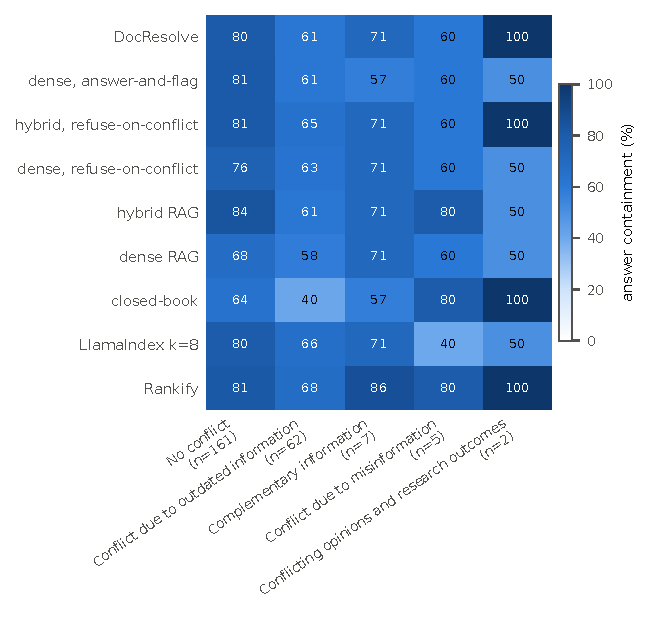
\includegraphics[width=\columnwidth]{fig_conflict_types}
  \caption{CONFLICTS accuracy by annotated conflict type and system (\genA).}
  \label{fig:types}
\end{figure}
\section{Example outputs}
\todo{One RAMDocs and one CONFLICTS item: question, retrieved values, the
system's decision and citations, next to plain RAG and refuse-on-conflict.}
\section{LLM-as-a-judge protocol}
\label{app:judge}
Every row is graded once by a single open-weight judge served locally with
vLLM, with greedy decoding and a 4\,096-token completion budget (reasoning
models may think; the \texttt{<think>} block is stripped before parsing).
The judge sees the question, the gold answer(s), the expected behaviour for
the situation, the system's decision label and its answer. It never sees the
retrieved documents, so it grades the answer, not the retrieval.
\todo{name the judge and report agreement with the earlier GLM judge on the
six shared rows and with gold on the labelled subset.}

\subsection{System prompt}
\begin{lstlisting}[style=prompt]
You are an impartial grader for a question-answering system that reads several retrieved documents, some of which may disagree. You compare the system's answer with the gold answer(s) and grade it with exactly one label:

FC  (fully correct): every gold answer is given as the answer, no incorrect value is presented as the answer or as an equally valid possibility, and the required behaviour for the situation is followed.
PC  (partially correct): the answer contains the gold answer(s) but is incomplete, hedges between the gold answer and an incorrect value without committing, or follows the required behaviour only partly. Nothing stated is factually wrong.
Inc (incorrect): the answer commits to an incorrect value, contradicts the gold answer, fails to give any gold answer, refuses or abstains although the gold answer was available, or clearly violates the required behaviour.

Grade substance only, not style or length. Minor differences in wording, formatting, units or precision that preserve the meaning do not count against the answer. Return JSON only, on one line: {"label": "FC" | "PC" | "Inc", "reason": "one sentence"}
\end{lstlisting}

\subsection{Per-item user turn, RAMDocs}
\begin{lstlisting}[style=prompt]
Question: <question>
Situation: the retrieved documents may mix correct information, misinformation and noise. If the question is ambiguous because several distinct entities share a name, each gold answer belongs to one entity and all of them must be given for FC. Known misinformation values are listed; presenting one of them as the answer is Inc, presenting it as an unresolved alternative alongside the gold answer is PC.
Gold answer(s): <gold 1> | <gold 2> | ...
Known misinformation value(s): <wrong 1> | <wrong 2> | ...
System decision label: <answered|unresolved_conflict|insufficient_evidence|needs_information>
System answer:
<predicted answer, or "(no answer given)">
Grade the system answer.
\end{lstlisting}

\subsection{Per-item user turn, CONFLICTS}
\begin{lstlisting}[style=prompt]
Question: <question>
Situation: <conflict type>. Required behaviour: <behaviour for that type, Table below>
Gold answer: <reference answer>   (or: "(no reference answer; grade the required behaviour and factual consistency with the situation only)")
System decision label: <decision>
System answer:
<predicted answer>
Grade the system answer.
\end{lstlisting}
The decision label line is omitted for the off-the-shelf frameworks, which
return free text.

\subsection{Expected behaviour per CONFLICTS conflict type}
These strings are the ones inserted into the judge prompt; the expected
decision is also the target of the automatic decision-match metric.
\begin{center}\small
\begin{tabular}{@{}p{0.27\columnwidth} p{0.14\columnwidth} p{0.5\columnwidth}@{}}
\toprule
Conflict type & Expected decision & Required behaviour given to the judge \\
\midrule
No conflict & answered & The sources agree; the response should give the single supported answer directly. \\
Complementary information & answered & The sources give different but compatible pieces of information (e.g.\ the answer differs by place, interpretation or sub-question); the response should answer by combining or distinguishing them rather than picking one and ignoring the rest. \\
Conflicting opinions and research outcomes & unresolved conflict & The sources genuinely disagree (opinions, contested research); the response should present the competing positions neutrally and not commit to one as the answer. \\
Conflict due to outdated information & answered & Some sources are out of date; the response should prefer the most recent information and give that as the answer, optionally noting that older sources differ. \\
Conflict due to misinformation & answered & Some sources are false; the response should ignore the misinformation and give the correct answer. \\
\bottomrule
\end{tabular}
\end{center}

\subsection{Parsing and bookkeeping}
The judge's reply is parsed as JSON after stripping code fences; a reply
without one of the three labels is retried and, if still unlabelled, counted
in \texttt{n\_unlabelled} and excluded from the percentages. Verdicts are
checkpointed per item, so an interrupted run resumes without re-grading.
Per-run summaries report FC / PC / Inc overall and broken down by conflict
type (CONFLICTS), by whether a reference answer exists, and by the system's
decision label.
\section{Hyperparameters and reproduction}
Generation: temperature 0, completion budget 16\,384 tokens, one repair call
at most. Judge: temperature 0, completion budget 4\,096 tokens. Retrieval:
BM25 and bge-small-en-v1.5 dense scores fused by reciprocal rank, 30
candidates, 8 chunks after diversification. Scoring weights: 0.3 semantic,
gate $\times$ (0.5 authority + 0.2 scope).
\todo{chunk sizes, model ids and endpoints for \genB{} and \genC{}, seeds,
and the \texttt{evaluate\_external.py} command line for every row.}

\end{document}
